\documentclass[jou]{apa6}

\usepackage[american]{babel}

\usepackage{csquotes}
\usepackage[style=apa,sortcites=true,sorting=nyt,backend=biber]{biblatex}
\DeclareLanguageMapping{american}{american-apa}
\addbibresource{bibliography.bib}


%%%%%%%%%%%%%%%%%%%%%%%%%%%%%%%%%%%%%%%%
%% Discrete Structures
%% The start of RBS stuff
%%%%%%%%%%%%%%%%%%%%%%%%%%%%%%%%%%%%%%%%

% Working internal and external links in PDF
\usepackage{hyperref}
% Extra math symbols in LaTeX
\usepackage{amsmath}
\usepackage{gensymb}
\usepackage{amssymb}
% Enumerations with (a), (b), etc.
\usepackage{enumerate}
\usepackage[framemethod=TikZ]{mdframed}
\usepackage{xcolor}
\usepackage{graphicx}
\usepackage[justification=centering]{caption}
\usepackage{fancyvrb}

\let\OLDitemize\itemize
\renewcommand\itemize{\OLDitemize\addtolength{\itemsep}{-6pt}}

\usepackage{etoolbox}
\makeatletter
\preto{\@verbatim}{\topsep=3pt \partopsep=3pt }
\makeatother

% These sizes redefine APA for A4 paper size
\oddsidemargin 0.0in
\evensidemargin 0.0in
\textwidth 6.27in
\headheight 1.0in
%\topmargin -24pt
\topmargin -32pt
\headheight 12pt
\headsep 12pt
%\textheight 9.19in
\textheight 9.35in


\title{Sample Quiz 8}
\author{Discrete Structures, Spring 2020}
\affiliation{RBS}

\leftheader{Discrete Sample Quiz 8}

\abstract{%
}

%\keywords{}

\setlength\parindent{0pt}

\begin{document}

%\thispagestyle{empty}

\twocolumn
\section{Final Topics and Sample Problems}

The final exam will contain two questions from 
each part \textendash{} 10 questions altogether. 
In this list of topics every part is subdivided
into several subtopics (and sample questions 
are mentioned for every subtopic). 
Therefore, the sample problems cover somewhat
larger range of topics than the actual final exam would.

\subsection{Part 1: Sets, Functions, Predicates and Quantifiers}

\subsubsection{1.1. Find the cardinality of sets}

{\bf Question:} {\em How many items are there?}\\
{\scriptsize
Count the number of elements or state that the set is (countably) infinite. 
We can define the sets using set operations (union, intersection, difference, 
symmetric difference), the images and inverse images of functions, 
set builder notation $\{ x \,\mid\, \text{where}\;x\;\text{satisfies}\;P(x)\}$, 
powersets and Cartesian products.\\
{\em Note:} We only deal with countable infinities. 
No need for the ``higher order infinities'', 
Cantor’s diagonalization or anything like this.
}


% Scheinerman; 12.2
\vspace{6pt}
{\bf Sample Problem 1.1.}\\
Let $A$ and $B$ be sets with sizes $|A| = 10$ and $|B| = 7$. Calculate 
the largest and the smallest possible values for each of the following expressions:\\
{\bf (A)} $|A \cap B| + |A \cup B|$,\\
{\bf (B)} $|A \times A \times B|$,\\
{\bf (C)} $\left| \mathcal{P}(A \cap B) \right|$,\\
{\bf (D)} $|A \oplus B|$.


\subsubsection{1.2. Check the subset relation between sets} 

{\bf Question:} {\em Does one condition imply another?}\\
{\scriptsize 
Given the definitions of two or more sets, establish, if sets are equal, 
or one of them is a (proper) subset of another. Use Euler-Venn diagrams 
showing set relations. Determine, if there is a logical implication 
in one direction (or in the opposite direction, or in both directions 
as in ``if and only if'' statements).
}

% Scheinerman; 10.11
\vspace{6pt}
{\bf Sample Problem 1.2.}\\
{\bf (A)} Let $a$ and $b$ be positive integers and let
\begin{equation}
\label{eq:set-notation-divisibility}
\left\{ \begin{array}{l}
A = \{ x \in \mathbb{Z}\;\mid\;a\mid{}x\},\\
B = \{ x \in \mathbb{Z}\;\mid\;b\mid{}x\}.
\end{array} \right.
\end{equation}
Find the necessary and sufficient condition for $A \subseteq B$. 

{\bf (B)} In the above definitions of the sets $A$, $B$ insert numbers
$a = 25$, $b = 40$. Write a simple definition for the set $C = A \cap B$. 

\vspace{4pt}
{\em Note.} In the formula (\ref{eq:set-notation-divisibility}) the first vertical 
bar is the part of set builder notation, the other vertical 
bar denotes the divisibility relation.



\subsubsection{1.3. Translate into predicates or quantifiers} 

{\bf Question:} {\em Can we formalize our thinking?}\\
{\scriptsize
Given an English statement (or other informal statement using tables, charts or function graphs) 
formalize this into expressions involving set notation, predicates and quantifiers. 
}


\vspace{6pt}
{\bf Sample Problem 1.3.}\\
Consider the following statement:
\begin{mdframed}[roundcorner=6pt]
Let $a_1,a_2,a_3,\ldots$ be a strictly increasing sequence of positive integers such that for any fixed positive integer $C$, the
sequence 
$$a_1+C, a_2+C, a_3 + C, \ldots$$
contains no more than a finite number of primes. 
\end{mdframed}

{\bf (A)} Rewrite the properties of the sequence $(a_n)$ predicates and quantifiers. 
You can use predicate $\text{isPrime}(n)$ that is {\tt true} iff $n$ is a prime. 
In your formula, $(a_n)$ is a {\em free variable} (somebody gave it to you), 
but all the other variables, if you need them,
should be {\em bound variables} \textendash{} the value of the formula should not depend on them.\\
{\bf (B)} Create a sequence $(a_n)$ that satisfies both conditions.






\subsubsection{1.4. Check properties of functions}

{\bf Question:} {\em Are there known patterns in functions?}\\
{\scriptsize 
Given a definition of sets and functions, verify, if they are injective, 
surjective, bijective. Also check, if functions are monotone 
(strictly or non-strictly increasing or decreasing) or constant. 
Build inverse functions and function compositions.
}

% Scheinerman, 24.21
\vspace{6pt}
{\bf Sample Problem 1.4.}\\
Let $f\,:A \rightarrow B$ be a function. We say that $f$ is {\em two-to-one}, if for
each $b \in B$ there are exactly two elements $a_1,a_2 \in A$ such that 
$f(a_1)=f(a_2) = b$.\\
It is known that $|A| = 2n$ and $|B| = n$ for some positive integer $n$. 
How many functions $f\,:A \rightarrow B$ are {\em two-to-one}?

\subsubsection{1.5. Partitions of a set} 

{\bf Question:} {\em When two different representations express the same object?}\\
{\scriptsize 
Given a set and some additional conditions, show how to define an equivalence 
relation that causes a partition of the set into equivalence classes. 
}


% Scheinerman, 16.17
\vspace{6pt}
{\bf Sample Problem 1.5.}\\
Let $A$ be a set with $100$ elements. We split $A$ into equivalence classes
(disjoint subsets $A_1,\ldots,A_n$ such that their union is $A$).\\
{\bf (A)} How many partitions of the set $A$ into $n=5$ parts of size $20$?\\
{\bf (B)} How many partitions of the set $A$ into $n=20$ parts of size $5$?\\



\newpage
\subsection{Part 2: Recursion, Sequences and Algorithms}

\subsubsection{2.1. Use iterative notation}

{\bf Question:} {\em How do we manipulate long expressions and the {\tt for} loops?}\\
{\scriptsize
Given formulas with $\sum_{i=1}^n\ldots$ (long summation), $\prod_{i=1}^n\ldots$ (long products), 
and big conjunctions, disjunctions, set unions, differences and symmetric differences, 
find out their meaning or compute the values. Also identify the iterative notation 
if you are given computer code that performs something or an expression with dots. 
Build interative definitions for sequences described in words \textendash{} 
number of ways to make change, counting strings with certain properties and so on.
}



% Scheinerman, p.70; selftest, 7
\vspace{6pt}
{\bf Sample Problem 2.1.}\\
{\bf (A)} Evaluate the following product:
$$\prod\limits_{k=0}^{100} \frac{k^2}{k+1}.$$
{\bf (B)} Evalue the following sum: 
$$\sum\limits_{k=1}^{100} \frac{1}{k(k+1)}.$$


\subsubsection{2.2. Use closed-form expressions for sequences}

{\bf Question:} {\em Can we describe a long procedure by a short formula?}\\
{\scriptsize
Given a description of a sequence (recurrent definition or some other), 
create the ``closed'' formula to compute its element. You can use 
characteristic equations, summation of arithmetic and 
geometric progressions, simple inductive reasoning to find them.
}

\vspace{6pt}
{\bf Sample Problem 2.2.}\\
Assume that the characteristic equation for a 
homogeneous linear recurrence relation with constant coefficients
is $(r-5)^3 = 0$. 

{\bf (A)} Write a recurrent definition of a sequence having this characteristic equation.\\
{\bf (B)} Describe the form for the general solution to the recurrence relation.



\subsubsection{2.3. Use mathematical induction}

{\bf Question:} {\em How do we prove anything about an infinite set?}\\
{\scriptsize 
Given a statement, describe the “inductive basis” and the ``inductive transition''. 
We can also have examples with Fibonacci-type sequences 
(where the inductive basis needs two statements instead of one), 
or ``strong induction'', where you may need the statement 
for all the previous values to make the next step.
}

\vspace{6pt}
{\bf Sample Problem 2.3.}\\
Given a positive integer $n$, consider the following sum with alternating signs:
$$S(n) = \sum\limits_{k=0}^{n-1} (-1)^k \cdot (n-k)^2.$$
For example, 
$$\left\{ \begin{array}{l}
S(1) = 1^2,\\
S(2) = 2^2 - 1^2,\\
S(3) = 3^2 - 2^2 + 1^2,\\
\ldots \\
S(n) = n^2 - (n-1)^2 + (n-2)^2 - \ldots + (-1)^{n-1} \cdot 1^2.\\
\end{array}
\right.$$

{\bf (A)} Find a closed expression for $S(n)$ (formula to calculate it without long summation).\\
{\bf (B)} Formulate the basis and the inductive transition of 
the mathematical induction proof.



\subsubsection{2.4. Write the Big-O-Notation} 

{\bf Question:} {\em How do we compare function growth and the speed of algorithms?}\\
{\scriptsize 
Given a description of an algorithm, a sequence or a real-valued function, 
define, which Big-O class this function belongs to; estimate the speed of its growth.
}


\vspace{6pt}
{\bf Sample Problem 2.4.}\\
Assume that you have a set $A$ with size $k$; this set contains 
words; all words have length $m$. An exhaustive search algorithm 
looks at all (ordered) pairs of elements $p_1,p_2 \in A$; 
it runs Knuth-Morris-Pratt algorithm (using $p_1$ as a pattern
and $p_2$ as a text). 

Write the time complexity of this exhaustive search algorithm 
(in terms of $k$ and $m$). Use Big-O-notation.


\subsubsection{2.5. Manipulate strings and finite lists}

{\bf Question:} {\em How to operate with a finite list of symbols.}\\
{\scriptsize 
Given a description of a string algorithm or another procedure, 
check its mathematical properties or build a counter-example. 
Same thing about finite lists of some other kind, for example, lists of integers. 
Use the concepts prefixes, suffixes, reverse strings, palindromes 
(strings that are the same from both ends), strings with balanced parentheses etc.
}

% Scheinerman, p.70, p.2
\vspace{6pt}
{\bf Sample Problem 2.5.}\\
In how many ways  can we make a list of three integers $(a,b,c)$ where 
$0 \leq a,b,c \leq 9$ and $a+b+c$ is even?


\newpage
\subsection{Part 3: Number Theory}

\subsubsection{3.1. Use divisibility, primes and factorization}

{\bf Question:} {\em How do the numeric properties depend on prime factorization?}\\
{\scriptsize 
Prove or disprove simple statements. List all divisors for a given number. 
Use reasoning that there are infinitely many primes.
}

\vspace{6pt}
{\bf Sample Problem 3.1.}\\
Let $A$ be the set of all positive divisors of the number $144$ 
(including $1$ and $144$ itself).\\
{\bf (A)} What is the multiplication of all 
numbers in the set $A$?\\
{\bf (B)} Express this number as the product of prime powers.


\subsubsection{3.2. Make computations in modular arithmetic}

{\bf Question:} {\em How to go from infinite sets to finite sets of congruence classes?}\\
{\scriptsize 
Given some statements involving remainders modulo m apply it for four 
arithmetic operations, polynomial values. 
Apply simple divisibility rules in form of congruence equations. 
}


\vspace{6pt}
{\bf Sample Problem 3.2.}
\begin{itemize}
\item ASCII value of {\tt h}: $c[\mathtt{h}]=104$,
\item ASCII value of {\tt e}: $c[\mathtt{e}]=101$,
\item ASCII value of {\tt y}: $c[\mathtt{y}]=121$.
\end{itemize}

Compute the Rabin-Karp hash values:\\
$H(\mathtt{hey}) = (c[\mathtt{h}] \cdot 257^2 + c[\mathtt{e}] \cdot 257 + c[\mathtt{y}] \cdot 257^0)\;\text{mod}\;29$,\\
$H(\mathtt{eyh}) = (c[\mathtt{e}] \cdot 257^2 + c[\mathtt{y}] \cdot 257 + c[\mathtt{h}] \cdot 257^0)\;\text{mod}\;29$,\\
$H(\mathtt{yhe}) = (c[\mathtt{y}] \cdot 257^2 + c[\mathtt{h}] \cdot 257 + c[\mathtt{e}] \cdot 257^0)\;\text{mod}\;29$.




\subsubsection{3.3. Use GCD, LCM and Bezout identity}

{\bf Question:} {\em What do we get by adding several arithmetic progressions?}\\
{\scriptsize 
Run Euclid’s algorithm to find GCD. Find LCM from GCD. Run Blankinship’s algorithm 
or to find the solution for the Bezout’s equation: $ax + by = d$, where $d = \text{gcd}(a,b)$. 
Find inverse values modulo $m$. Apply this to individual linear congruences 
or simple systems (as in Chinese Remainder Theorem).
}

\vspace{6pt}
{\bf Sample Problem 3.4.}\\
Somebody wants to find two subsequent numbers such that 
none of them can be expressed as a power $n^k$ (where $k>1$). 
To be sure that none of them is a power, s/he creates the following system: 
$$\left\{ \begin{array}{l} 
x \equiv 2\,(\text{mod}\;2^2)\\
x+1 \equiv 3\,(\text{mod}\;3^2)\\
\end{array} \right.$$
{\bf (A)} Find a solution for this system.\\
{\bf (B)} Find a solution for a larger system (it would give a sequence of three
subsequent numbers): 
$$\left\{ \begin{array}{l} 
x \equiv 2\,(\text{mod}\;2^2)\\
x+1 \equiv 3\,(\text{mod}\;3^2)\\
x+2 \equiv 5\,(\text{mod}\;5^2)\\
\end{array} \right.$$



\subsubsection{3.4. Number notation in other bases}

{\bf Question:} {\em How to express numbers as polynomials with different bases?}\\
{\scriptsize 
Convert numbers from one base into another. Use infinite geometric progression 
summation and other ways to manipulate the numbers (including fractions) 
in binary and other simple bases. Use the relationship between 
the logarithm of the number and the length of its notation.
}

\vspace{6pt}
{\bf Sample Problem 3.4.}\\
Create an example of a rational number having an infinite binary representation: 
$$\beta = 0.b_1b_2b_3b_4b_5b_6b_7\ldots,$$
where the bits have period $T = 10$, i.e. $b_1 = b_{11}$, $b_2 = b_{12}$, etc. 
(Your number $\beta$ should not have any periods shorter than $10$.)



\subsubsection{3.5. Repetitive Processes in Number Theory} 

{\bf Question:} {\em What happens, if the same operation is done again and again?}\\
{\scriptsize 
Describe a fast variant of modular exponentiation. 
Estimate when there should be an infinite loop. Use the Fermat’s and Euler’s theorems. 
How this affects ``primitive roots'', the number of digits in periodic decimal fractions and so on. 
}


\vspace{6pt}
{\bf Sample Problem 3.5.}\\
Consider a sequence
$$\left\{ \begin{array}{l}
a_1 = 1\\
a_{n+1} = (2a_n + 3)\;\text{mod}\;17\\
\end{array} \right.$$

{\bf (A)} Write the members of this sequence until they start to repeat.\\
{\bf (B)} What is the period of this sequence?\\
{\bf (C)} Can we pick a different initial value $a_1$ so that the sequence will 
have a ``pre-periodic phase'' (i.e. before the period repeat starts, there 
are some values that lead to the period).




\newpage
\subsection{Part 4: Counting and Probabilities}

\subsubsection{4.1. Compute combinations and probabilities}

{\bf Question:} {\em How to count items taking into account their symmetries?}\\
{\scriptsize 
Given a description of a set or a tree-like decision process, 
count the variants using multiplication rule and its variants. 
Also addition, subtraction or division rules \textendash{} to ensure that 
everything is counted exactly once. 
Count set union sizes using inclusion-exclusion principle.
}

% Scheinerman, 8.1 (var)
\vspace{6pt}
{\bf Sample Problem 4.1.}\\ 
{\bf (A)} There are $5$ alphabetically sorted vowels $\{ A, E, I, O, U \}$. 
How many $3$-letter words one can create that can contain equal letters, 
but all letters are in increasing alphabetical order. 
(For example, ``words'' $AAA$, $AUU$ and $IOU$ are legal, but $EAI$ is not.)\\
{\bf (B)} Write all such words that start with letter $I$ \textendash{} 
arrange them in alphabetical order.

\subsubsection{4.2. Use Pigeonhole principle} 

{\bf Question:} {\em How should pigeons collide for the given counts of pigeons and holes?}\\
{\scriptsize 
Verify, if there can be bijective (or injective) 
mapping between some two sets. Combine with other combinatorial 
methods to find out, how uniqueness of identifiers can be ensured.
}


% Scheinerman, 25.7
\vspace{6pt}
{\bf Sample Problem 4.2.}\\ 
{\bf (A)} Find the smallest number $N$, 
such that among any $N$ positive integers 
there are at least $5$ numbers ending with the same digit.\\
{\bf (B)} Given a set of seven distinct positive integers, 
prove that there is a pair whose sum or whose
difference is a multiple of $10$.




\subsubsection{4.3. Use factorials and binomial coefficients} 

{\bf Question:} {\em How to combine multiple choices from the same set?}\\
{\scriptsize 
Compute combinations with or without repetitions. Use binomial formula with its coefficients. 
}

% Scheinerman, 17.3
\vspace{6pt}
{\bf Sample Problem 4.3.}\\
{\bf (A)} What is the coefficient of $x^3$ in $(1 + x)^6$? \\
{\bf (B)} What is the coefficient of $x^3$ in $(2x - 3)^6$?\\
{\bf (C)} What is the coefficient of $x^3$ in $(x + 1)^{20} + (x-1)^{20}$? \\
{\bf (D)} What is the coefficient of $x^3y^3$ in $(x+y)^6$? \\
{\bf (E)} What is the coefficient of $x^3y^3$ in $(x+y)^7$?

\subsubsection{4.4. Use independent events and Bayes formula}

{\bf Question:} {\em What does a new event add to our knowledge about 
the probabilities of other events?}\\
{\scriptsize 
What events are considered independent? 
What is a conditional probability. 
Switch the order in the conditional probability, using Bayes formula. 
}


% Scheinerman, 17.3
\vspace{6pt}
{\bf Sample Problem 4.4.}\\
About $40\%$ of all librarians 
and also about $10\%$ of all ``Rimi'' shop 
assistants like to read books by R.Blaumanis. 
For every librarian there are $20$ ``Rimi'' 
shop assistants.

Assume that you know that some person $x$ is either a
librarian or a ``Rimi'' shop assistant; and you also know that
s/he likes to read books by R.Blaumanis. 
Find the probability that $x$ is a librarian.



\subsubsection{4.5. Use random variables, expected value, variance}

{\bf Question:} {\em How to summarize complex probability distributions with just 2 numbers?}\\
{\scriptsize
Identify random variables from ``word problems'', descriptions of real-world situations.
For the given random variable $X$ compute $E(X)$ and $V(X)$. Use Markov's and Chebyshev's 
inequalities.
}


\vspace{6pt}
{\bf Sample Problem 4.5.}\\
Let $Q_5$ be the $5$-dimensional hypercube with $32$ vertices. 
Let $X$ be a random variable that is obtained as follows:\\
Select two different random vertices $v_1,v_2$ in $Q_5$. Set $X=1$, 
if $v_1,v_2$ are connected with an edge. 

{\bf (A)} Find $E(X)$. \\
{\bf (B)} Find $V(X)$. 





\newpage
\subsection{Part 5: Graphs and Trees}

\subsubsection{5.1. Verify and use relation properties}

{\bf Question:} {\em How relations relate to directed graphs?}\\
{\scriptsize
Check, if a relation is reflexive, symmetric, transitive, antisymmetric. Find relation joins and powers. Show relations as directed graphs or read them from graphs. Use total and partial order relationships.
}



% Scheinerman; 14.3
\vspace{6pt}
{\bf Sample Problem 5.1.}\\
For each of the following relations defined on the set $\{ 1,2,3,4,5 \}$ determine whether
the relation is reflexive, symmetric, antisymmetric, and/or transitive. 


{\bf (A)} $R = \{ (1,1), (2,2), (3,3), (4,4), (5,5) \}$,\\
{\bf (B)} $R = \{ (1,1), (2,1), (2,2), (3,1), (3,2), (3,3), (4,1),$\\
\mbox{}$\;\;(4,2),(4,3), (4,4), (5,1), (5,2), (5,3), (5,4), (5,5) \}$,\\
{\bf (C)} $R = \{ (1,2), (2,3), (3,4), (4,5) \}$,\\
{\bf (D)} $R = \{ (1,1), (1,2), (1,3), (1,4), (1,5) \}$,\\
{\bf (E)} $R = \{ (1,1), (1,2), (2,1), (3,4), (4,3) \}$,\\
{\bf (F)} $R = \{ 1,2,3,4,5 \} \times \{ 1,2,3,4,5 \}$. 

Enter the truth values in a table: 

\begin{tabular}{|l|c|c|c|c|} \hline
{\scriptsize Question} & {\scriptsize Reflexive} & {\scriptsize Symmetric} & {\scriptsize Antisymmetric} & {\scriptsize Transitive} \\ \hline
{\bf (A)} & & & & \\ \hline
{\bf (B)} & & & & \\ \hline
{\bf (C)} & & & & \\ \hline
{\bf (D)} & & & & \\ \hline
{\bf (E)} & & & & \\ \hline
{\bf (F)} & & & & \\ \hline
\end{tabular}



\subsubsection{5.2. Create graphs and count graph elements}

{\bf Question:} {\em How to translate problems into graph notation?}\\
{\scriptsize 
Create a graph from non-graph problems. Find vertex/edge counts or verify 
simple properties for simple undirected and directed graphs. Build some known types of graphs 
($K_n$ \textendash{} full graph, $C_n$ \textendash{} cyclic graph, 
$W_n$ \textendash{} wheel graph, $Q_n$ \textendash{} $n$-dimensional hypercube.) 
Use adjacency and incidence matrices.
}






% Scheinerman; 49.10
\vspace{6pt}
{\bf Sample Problem 5.2.}\\
Let $G$ be a simple undirected graph. Prove that $G$ or $\overline{G}$ (or both) must be connected.\\
{\em Note.} Graph $\overline{G}$ is the {\em complement} of the graph $G$; it is formed by removing all the edges of 
$G$ and replacing them by all possible edges that are not in $G$. 

\subsubsection{5.3. Check graph properties} 

{\bf Question:} {\em How to verify and use basic graph properties?}\\
{\scriptsize 
Verify connectivity, cyclic or acyclic graphs, Euler and Hamilton paths, 
graph planarity and colorings. For graphs defined by their adjacency matrices 
or implicit definitions check, if the graph is connected/disconnected, 
cyclic/acyclic, contains paths of certain kinds, 
can be isomorphic to a planar graph or a 3D solid. 
}


% Scheinerman; 
\vspace{6pt}
{\bf Sample Problem 5.3.}\\
Graph $G$ is defined by the following adjacency matrix:
$$M_G = \left(
\begin{array}{ccccccc}
0 & 1 & 1 & 0 & 0 & 0 & 0 \\
1 & 0 & 0 & 1 & 1 & 0 & 0 \\
1 & 0 & 0 & 0 & 0 & 1 & 1 \\
0 & 1 & 0 & 0 & 0 & 0 & 0 \\
0 & 1 & 0 & 0 & 0 & 0 & 0 \\
0 & 0 & 1 & 0 & 0 & 0 & 0 \\
0 & 0 & 1 & 0 & 0 & 0 & 0 \\
\end{array} \right).$$

{\bf (A)} Is graph $G$ connected?\\
{\bf (B)} Is graph $G$ cyclic?\\
{\bf (C)} Does $G$ have a Euler path?

Justify your answers.



\subsubsection{5.4. Use DFS and BFS tree traversal algorithms} 

{\bf Question:} {\em What are some orderly ways to list vertices that are broadly applicable?}\\
{\scriptsize 
Given a simple directed or undirected graph find the traversal order. 
Restore a tree from its traversal order. Rewrite expressions and their syntax trees in preorder, inorder, postorder ways.
}



% Scheinerman; 49.10
\vspace{6pt}
{\bf Sample Problem 5.4.}
\begin{figure}[!htb]
\center{\includegraphics[width=3in]{final-exam-preparation/perfect-binary-tree.png}}
\caption{\label{fig:perfect-binary-tree} A perfect binary tree.}
\end{figure}


In the perfect binary tree (Figure~\ref{fig:perfect-binary-tree}) all leaves are at the level $4$. 
All nodes in this tree are enumerated in the BFS order (using numbers from $1$ to $31$). 
Let $s_1,\ldots,s_{31}$ be the sequence of numbers that is created when doing in-order DFS traversal of this tree. 

{\bf (A)} Find the sum $s_1 + s_3 + \ldots + s_{31}$ (add all the odd numbers in this sequence).\\
{\bf (B)} Find the sum $s_2 + s_4 + \ldots + s_{30}$ (add all the odd numbers in this sequence).\\


\subsubsection{5.5. Use Prim's and Dijkstra's algorithms}

{\bf Question:} {\em How to solve practical tasks in weighted graphs and transport networks?}\\
{\scriptsize 
Given a weighted undirected graph, find the shortest path or the minimum spanning tree. 
Check simple statements about the spanning trees and shortest paths. 
}





\vspace{6pt}
{\bf Sample Problem 5.5.}\\ For the graph on Figure~\ref{fig:dijkstra-graph} 
find the shortest paths from the vertex $A$ 
to all the other vertices. For each vertex $B,C,D,E,F$ write the total length of the 
shortest path and also the step in the Dijkstra's tree-growing algorithm at which you added that vertex. 

\begin{figure}[!htb]
\center{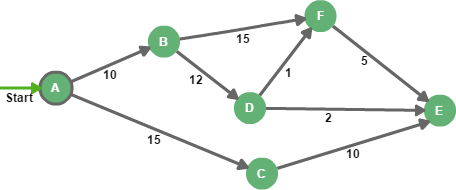
\includegraphics[width=3in]{final-exam-preparation/dijkstra-graph.png}}
\caption{\label{fig:dijkstra-graph} A weighted graph.}
\end{figure}

\begin{tabular}{|l|c|c|} \hline
Vertex & Mininum Path & Step number \\ \hline
$B$ & & \\ \hline
$C$ & & \\ \hline
$D$ & & \\ \hline
$E$ & & \\ \hline
$F$ & & \\ \hline
\end{tabular}


\end{document}

